\section{Przedstawienie danych statystycznych}

% ------------------------------------------------------------------------------
% Slide 1: Struktura Mocy Zainstalowanej w Polsce
% ------------------------------------------------------------------------------
\begin{frame}{Struktura mocy zainstalowanej w Polsce (31.12.2024)}
    \begin{columns}[T]
        % Lewa kolumna: Tabela z danymi
        \begin{column}{0.5\textwidth}
            \includetable{installed_capacity}
        \end{column}
        
        % Prawa kolumna: Wykres kołowy
        \begin{column}{0.5\textwidth}
            \includefigure{installed_power_structure}
        \end{column}
    \end{columns}
    
    \begin{tcolorbox}[colback=renewable!10, colframe=renewable!80!black, title=Kluczowy wniosek]
        \faIcon{leaf} \textbf{Dominacja OZE:} Odnawialne źródła energii, głównie wiatrowe i fotowoltaiczne, stanowią obecnie największy udział w całkowitej mocy zainstalowanej w Polsce, co świadczy o dynamicznej transformacji energetycznej.
    \end{tcolorbox}
\end{frame}

% ------------------------------------------------------------------------------
% Slide 2: Rozwój Mocy na Przestrzeni Lat
% ------------------------------------------------------------------------------
\begin{frame}{Moc zainstalowana w Polsce na przestrzeni lat [MW]}
    \begin{columns}[T]
        % Lewa kolumna: Wykres liniowy
        \begin{column}{0.6\textwidth}
            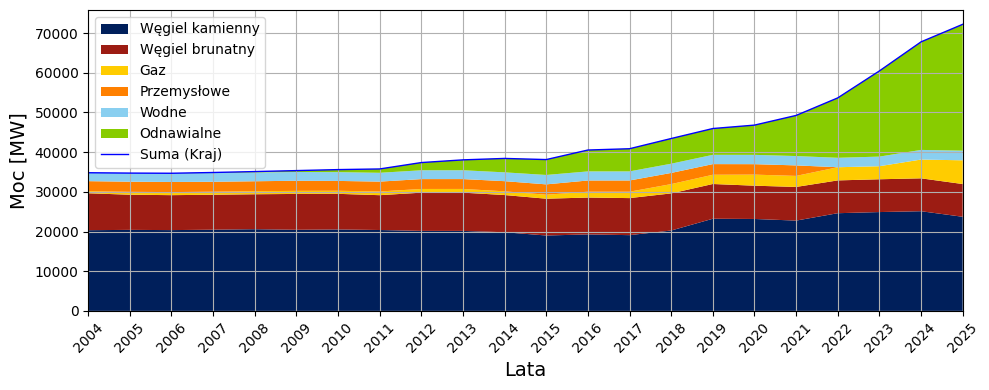
\includegraphics[width=\textwidth]{images/powerOverYears.png}
        \end{column}
        
        % Prawa kolumna: Wnioski
        \begin{column}{0.4\textwidth}
            \vspace{1cm} % Dodanie przestrzeni dla lepszego wyrównania
            \begin{itemize}
                \item[\faIcon{chart-line}] \highlight{Dynamiczny wzrost:} W ostatnich latach obserwujemy wykładniczy przyrost mocy zainstalowanej ze źródeł odnawialnych.
                \item[\faIcon{wind}] \highlight{Lider transformacji:} OZE to obecnie najszybciej rozwijający się segment polskiej energetyki.
            \end{itemize}
        \end{column}
    \end{columns}
\end{frame}

% ------------------------------------------------------------------------------
% Slide 3: Porównanie Europejskie - Udział OZE i Energii Nuklearnej
% ------------------------------------------------------------------------------
\begin{frame}{Udział OZE i energii nuklearnej w produkcji energii (2023)}
    \begin{columns}[T]
        % Lewa kolumna: Tabela porównawcza
        \begin{column}{0.5\textwidth}
             \includetable{OZE_percentage}
        \end{column}

        % Prawa kolumna: Wykres słupkowy
        \begin{column}{0.5\textwidth}
            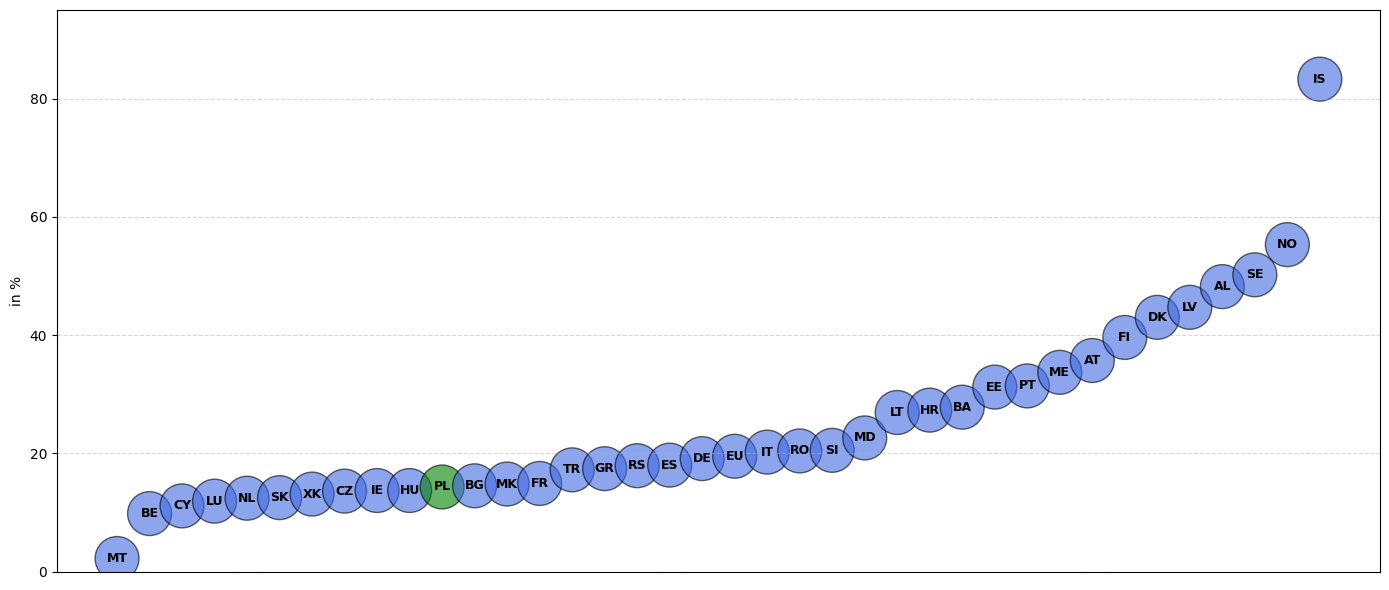
\includegraphics[width=\textwidth]{images/ozePercentageShare.png}
        \end{column}
    \end{columns}
    \begin{itemize}
        \item \small \highlight{Paradoks mocy a produkcja:} Mimo dużego udziału w mocy zainstalowanej, realny wkład OZE w produkcję energii w Polsce jest wciąż relatywnie niski w porównaniu do liderów europejskich.
        \item \small \highlight{Strategie mieszane:} Wiele krajów europejskich skutecznie łączy wysoki udział OZE z energią nuklearną, aby zapewnić stabilność i niskie emisje.
    \end{itemize}
\end{frame}

% ------------------------------------------------------------------------------
% Slide 4: Emisje CO2 w Europie
% ------------------------------------------------------------------------------
\begin{frame}{Emisje CO\textsubscript{2} na mieszkańca w Europie (2023)}
    \includetable{co2_emissions}
\end{frame}

% ------------------------------------------------------------------------------
% Slide 5: Ceny Energii w Polsce na przestrzeni lat
% ------------------------------------------------------------------------------
\begin{frame}{Cena energii dla gospodarstw domowych w Polsce (z uwzględnieniem podatków)}
    \begin{columns}
        % Lewa kolumna: Wykres słupkowy
        \begin{column}{0.6\textwidth}
            \includefigure{EnergyPriceOverYears}
        \end{column}
        
        % Prawa kolumna: Główne obserwacje
        \begin{column}{0.4\textwidth}
             \begin{tcolorbox}[colback=coalplant!10, colframe=coalplant!80!black, title=Kluczowe obserwacje]
                \begin{itemize}
                    \item[\faIcon{arrow-up}] \textbf{Tendencja wzrostowa:} Ceny energii dla gospodarstw domowych w Polsce systematycznie rosną.
                    \item[\faIcon{exclamation-triangle}] \textbf{Rekordowy rok 2024:} Ostatni rok przyniósł najwyższe historycznie ceny, co stanowi wyzwanie dla konsumentów.
                \end{itemize}
            \end{tcolorbox}
        \end{column}
    \end{columns}
\end{frame}

% ------------------------------------------------------------------------------
% Slide 6: Porównanie Cen Energii w Europie
% ------------------------------------------------------------------------------
\begin{frame}{Porównanie cen energii w Europie (PPS, 2023)}
    \includetable{energy_prices}
\end{frame}

% ------------------------------------------------------------------------------
% Slide 7: Zależność Energetyczna
% ------------------------------------------------------------------------------
\begin{frame}{Zależność energetyczna od importu w Europie (2023)}
    \includetable{import_dependency}
\end{frame}
